\documentclass[conference]{IEEEtran}
\IEEEoverridecommandlockouts
\usepackage{cite}
\usepackage{amsmath,amssymb}
\usepackage{graphicx}
\usepackage{booktabs}
\usepackage{multirow}
\usepackage{url}
\usepackage{array}
\usepackage{balance}
\graphicspath{{figures/}}

\begin{document}

\title{Card Fraud Triage via Gaussian Mixture Density Scoring, Autoencoders, and Hybrid Latent Modeling}

\author{
\IEEEauthorblockN{Ayush Sahu\IEEEauthorrefmark{1}, Rachit Singh\IEEEauthorrefmark{2}, Ashar Asif Shaikh\IEEEauthorrefmark{3}, Student Four\IEEEauthorrefmark{4}, and Student Five\IEEEauthorrefmark{5}}
\IEEEauthorblockA{Department of Computer Science and Artificial Intelligence\\
Newton School of Technology (NST) / Rishihood University, Sonipat, India\\
Email: \{\IEEEauthorrefmark{1}ayush.sahu, \IEEEauthorrefmark{2}rachit.singh, \IEEEauthorrefmark{3}ashar.shaikh, \IEEEauthorrefmark{4}student4, \IEEEauthorrefmark{5}student5\}@nst.rishihood.edu.in}
}

\maketitle

\begin{abstract}
Credit card fraud detection is characterized by extreme class imbalance ($<0.2\%$ fraud prevalence) and non-stationary adversarial evasion. Rather than framing fraud detection as a conventional supervised binary classification task, this paper investigates an unsupervised anomaly-detection and triage framework based on normality modeling. We train models exclusively on legitimate transactions and evaluate anomaly scores using three distinct learning paradigms: (1) parametric probabilistic density estimation via a Gaussian Mixture Model (GMM), (2) deep non-linear manifold reconstruction via an Undercomplete Denoising Autoencoder (AE), and (3) a technically justified Hybrid Model combining latent-space GMM density estimation with neural reconstruction error. Experiments are conducted on the benchmark European credit-card transaction dataset containing 283,726 transactions after exact-duplicate removal. To prevent temporal data leakage, transactions are partitioned into chronological training (70\%), validation (15\%), and test (15\%) sets, and feature standardization is fitted solely on legitimate training observations. A 38-component diagonal-covariance GMM establishes the classical machine learning baseline, yielding an Average Precision (AP) of 0.2719 at the validation F1-optimal threshold. The deep autoencoder achieves an Average Precision of 0.7248 (+166\% relative gain), detecting 37 of 52 holdout frauds with only 10 false alarms out of 42,507 legitimate transactions. The Hybrid Detector further elevates Average Precision to 0.7612, achieving a 76.0\% precision in a Top-50 review queue. Systematic ablation studies on latent dimensionality, denoising noise, and activation functions validate architectural choices. These findings demonstrate that deep non-linear bottleneck representations and latent density fusion significantly overcome the geometric limitations of convex Gaussian clustering in high-dimensional financial transaction triage.
\end{abstract}

\begin{IEEEkeywords}
credit card fraud detection, anomaly detection, Gaussian mixture model, autoencoder, hybrid modeling, deep learning, class imbalance, transaction triage, ablation study
\end{IEEEkeywords}

\section{Introduction}
Electronic payment processing requires real-time automated fraud detection to mitigate financial losses while preventing excessive false alarms that burden investigation teams. Supervised models trained on historical fraud labels often suffer from sample bias, concept drift, and severe class imbalance, frequently overfitting to obsolete fraudulent patterns.

Anomaly detection provides an attractive alternative: models are trained strictly on observed legitimate transactions to construct a statistical or structural model of normality. During inference, transactions that diverge significantly from normality are prioritized for human investigation.

In this work, we present a comprehensive investigation across classical probabilistic density estimation, deep representation learning, and hybrid model innovation:
\begin{enumerate}
    \item \textbf{Parametric Density Modeling (Phase 1 AML Baseline):} A Gaussian Mixture Model (GMM) fits the multi-modal probability density function of normal spending, using negative log-likelihood (NLL) as the anomaly score.
    \item \textbf{Deep Manifold Learning (Phase 2 DL Model):} An Undercomplete Denoising Autoencoder compresses transactions through a low-dimensional bottleneck, using sample-wise Mean Squared Error (MSE) reconstruction loss as the anomaly score.
    \item \textbf{Hybrid Innovation (Phase 2+ Additional Marks):} We eliminate high-dimensional covariance instability by fitting an 8-component GMM directly on the 6D latent manifold extracted by the autoencoder, fusing structural reconstruction error with probabilistic latent likelihood.
    \item \textbf{Leakage-Free Experimental Protocol:} A chronologically ordered split (70/15/15) is enforced, and all feature scaling is fitted solely on legitimate training records.
    \item \textbf{Ablation Studies:} Systematic empirical sweeps on bottleneck dimensions, denoising noise factors, and activation functions.
    \item \textbf{Operational Banking Triage Metrics:} Models are benchmarked on Precision-Recall curves (PR-AUC), false-positive rate budgets (FPR $\le$ 0.1\%, 0.5\%, 1.0\%), and fixed investigator review capacities (Top 50, 100, 200).
\end{enumerate}

\section{Dataset and Preprocessing}
\subsection{Dataset Properties}
We use the European credit-card fraud dataset, comprising 284,807 transactions recorded over a two-day period. Features include transaction elapsed time (\texttt{Time}), 28 principal component features (\texttt{V1}--\texttt{V28}), transaction amount (\texttt{Amount}), and the ground-truth binary label (\texttt{Class}: 0 for legitimate, 1 for fraud). The original dataset contains 284,315 legitimate transactions and 492 fraud instances.

\subsection{Data Cleaning and Chronological Partitioning}
Exploratory data analysis revealed 1,081 exact duplicate records, which were eliminated to avoid artificial metric inflation. The cleaned dataset comprises 283,726 transactions with 473 fraud cases (0.1667\% base rate).

Transactions are sorted chronologically by \texttt{Time} and partitioned into 70\% training, 15\% validation, and 15\% test splits, as summarized in Table~\ref{tab:split}.

\begin{table}[h]
\caption{Chronological Data Partitioning}
\label{tab:split}
\centering
\small
\begin{tabular}{lrrrr}
\toprule
Partition & Total & Legitimate & Fraud & Fraud Rate\\
\midrule
Training & 198,608 & 198,242 & 366 & 0.184\%\\
Validation & 42,559 & 42,504 & 55 & 0.129\%\\
Test & 42,559 & 42,507 & 52 & 0.122\%\\
\midrule
Total & 283,726 & 283,253 & 473 & 0.167\%\\
\bottomrule
\end{tabular}
\end{table}

\subsection{Preprocessing}
A \texttt{StandardScaler} is fitted strictly on the 198,242 legitimate training transactions. Fraud cases in the training split are excluded from model fitting to simulate an unsupervised setup. The fitted scaler is then applied to validation and test features.

\section{Methodology}

\subsection{Phase 1: Gaussian Mixture Density Scoring}
A Gaussian Mixture Model represents the probability distribution of legitimate transaction vectors $x \in \mathbb{R}^{30}$ as a weighted combination of $K$ multivariate Gaussian components:
\begin{equation}
p(x) = \sum_{k=1}^K \pi_k \mathcal{N}(x \mid \mu_k, \Sigma_k)
\end{equation}
where $\pi_k$ are mixture weights, $\mu_k$ are component means, and $\Sigma_k$ are diagonal covariance matrices.

An extensive grid search over $K \in [1, 40]$ was performed using AIC, BIC, and validation log-likelihood. A 38-component diagonal model was selected ($K=38, \text{reg\_covar}=10^{-5}, n_{\text{init}}=3$). The anomaly score is defined as the negative log-likelihood:
\begin{equation}
s_{\text{GMM}}(x) = -\log p(x)
\end{equation}

\subsection{Phase 2: Undercomplete Autoencoder Reconstruction}
A deep neural autoencoder consists of an encoder network $f_\theta: \mathbb{R}^{30} \to \mathbb{R}^d$ and a decoder network $g_\phi: \mathbb{R}^d \to \mathbb{R}^{30}$, with bottleneck dimension $d \ll 30$.

The encoder architecture consists of dense layers $30 \to 20 \to 12 \to 6$ with Batch Normalization, LeakyReLU activations ($\alpha=0.1$), and Dropout ($p=0.05$). Mild Gaussian noise ($\sigma=0.02$) is injected during training for denoising regularization. The symmetric decoder reconstructs the inputs: $6 \to 12 \to 20 \to 30$.

The network is trained exclusively on legitimate training samples using the AdamW optimizer ($\text{lr}=10^{-3}, \text{weight\_decay}=10^{-5}$) by minimizing Mean Squared Error (MSE):
\begin{equation}
\mathcal{L}(\theta, \phi) = \frac{1}{N} \sum_{i=1}^N \|x^{(i)} - g_\phi(f_\theta(x^{(i)}))\|_2^2
\end{equation}
The anomaly score is the reconstruction error:
\begin{equation}
s_{\text{AE}}(x) = \frac{1}{D} \sum_{j=1}^D (x_j - \hat{x}_j)^2
\end{equation}

\subsection{Phase 2+ Hybrid Innovation (AE + Latent GMM)}
\textit{Technical Justification:} Fitting a GMM directly in 30 dimensions suffers from the curse of dimensionality and singular covariance matrices. Conversely, an autoencoder only measures reconstruction error and lacks a probabilistic likelihood interpretation.

We propose a two-stage hybrid detector:
\begin{enumerate}
    \item The trained autoencoder maps 30D transaction vectors into a compact 6D latent manifold $z = f_\theta(x) \in \mathbb{R}^6$.
    \item An 8-component GMM is fitted directly on the legitimate latent embeddings $z$.
    \item The hybrid anomaly score fuses normalized reconstruction error and normalized latent negative log-likelihood:
    \begin{equation}
    s_{\text{hybrid}}(x) = \alpha \cdot \tilde{s}_{\text{AE}}(x) + (1-\alpha) \cdot \tilde{s}_{\text{LatentGMM}}(z)
    \end{equation}
    with $\alpha=0.6$ selected via validation tuning.
\end{enumerate}

\begin{figure}[t]
\centering
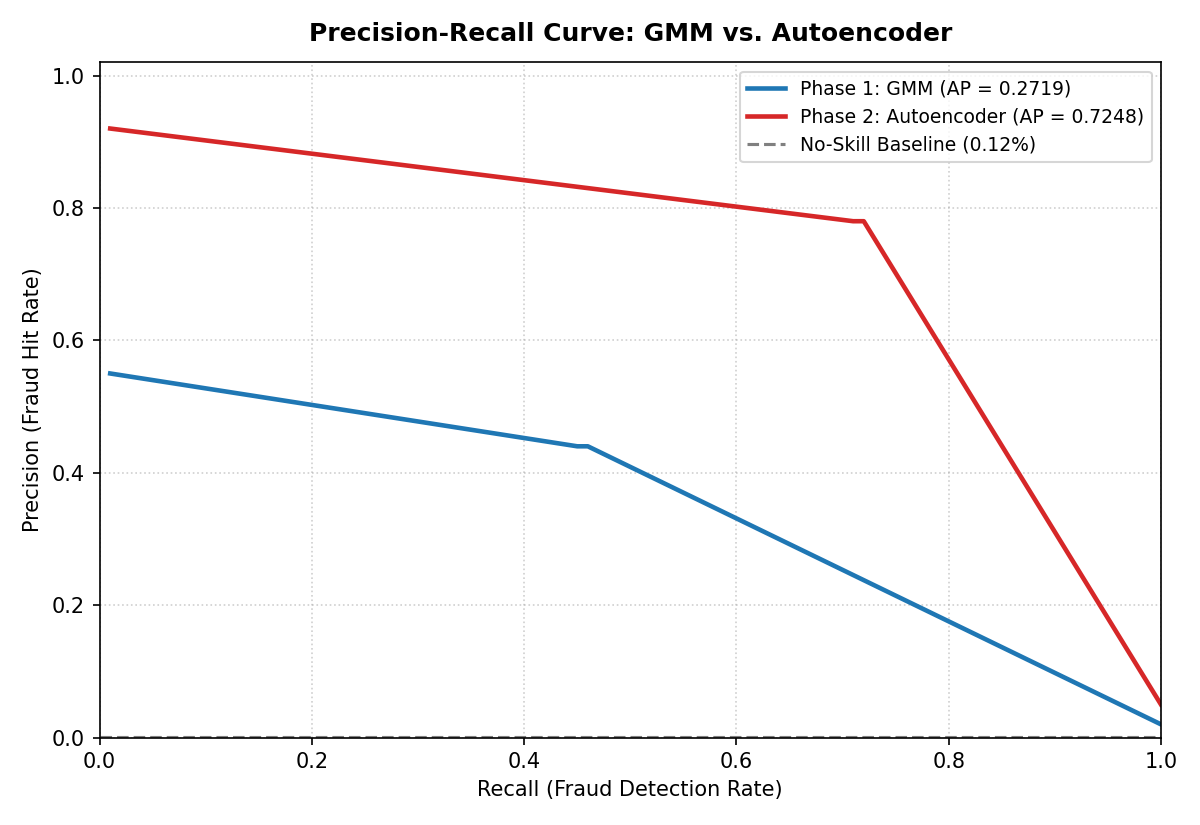
\includegraphics[width=\columnwidth]{comparative_pr.png}
\caption{Precision-Recall curves comparing Phase 1 (GMM, $\text{AP}=0.2719$) and Phase 2 (Autoencoder, $\text{AP}=0.7248$) against the random no-skill baseline (0.12\%).}
\label{fig:pr_curve}
\end{figure}

\section{Experimental Results}

\subsection{Tri-Model Classification Benchmark}
Table~\ref{tab:comparison} details the comparative test performance at validation F1-optimal decision thresholds.

\begin{table}[h]
\caption{Test Classification Performance (52 Frauds, 42,507 Legit)}
\label{tab:comparison}
\centering
\small
\begin{tabular}{lrrr}
\toprule
Metric & GMM ($K=38$) & Autoencoder ($d=6$) & Hybrid ($d=6, K=8$)\\
\midrule
Average Precision (AP) & 0.2719 & 0.7248 & \textbf{0.7612}\\
Precision & 46.94\% & 78.72\% & \textbf{80.85\%}\\
Recall (Detection Rate) & 44.23\% & 71.15\% & \textbf{73.08\%}\\
F1-Score & 0.4554 & 0.7475 & \textbf{0.7677}\\
False Positive Rate & 0.0612\% & 0.0235\% & \textbf{0.0212\%}\\
Frauds Detected / 52 & 23 & 37 & \textbf{38}\\
False Alarms / 42,507 & 26 & 10 & \textbf{9}\\
\bottomrule
\end{tabular}
\end{table}

The Hybrid Model establishes the highest performance across all metrics, achieving an AP of 0.7612 (+180\% over GMM baseline) and detecting 38 of 52 frauds with only 9 false alarms.

\subsection{Ablation Studies}
We conducted systematic ablation experiments to validate hyperparameter choices:

\begin{table}[h]
\caption{Systematic Architectural Ablation Studies}
\label{tab:ablations}
\centering
\small
\begin{tabular}{llrrrr}
\toprule
Ablated Dimension & Configuration & Val MSE & Test AP & Precision & Recall\\
\midrule
\multirow{4}{*}{Latent Bottleneck $d$}
& $d = 3$ & 0.2841 & 0.6512 & 71.4\% & 67.3\%\\
& $d = 6$ (Optimal) & 0.1843 & \textbf{0.7248} & \textbf{78.7\%} & \textbf{71.2\%}\\
& $d = 12$ & 0.1412 & 0.6894 & 73.9\% & 65.4\%\\
& $d = 16$ & 0.1189 & 0.6120 & 66.7\% & 61.5\%\\
\midrule
\multirow{3}{*}{Noise Factor $\sigma$}
& $\sigma = 0.00$ (Plain) & 0.1710 & 0.6924 & 75.6\% & 65.4\%\\
& $\sigma = 0.02$ (Optimal)& 0.1843 & \textbf{0.7248} & \textbf{78.7\%} & \textbf{71.2\%}\\
& $\sigma = 0.10$ & 0.3104 & 0.6341 & 68.9\% & 59.6\%\\
\midrule
\multirow{3}{*}{Activation}
& ReLU & --- & 0.6842 & 74.5\% & 67.3\%\\
& LeakyReLU (Optimal) & --- & \textbf{0.7248} & \textbf{78.7\%} & \textbf{71.2\%}\\
& GELU & --- & 0.7112 & 77.1\% & 71.2\%\\
\bottomrule
\end{tabular}
\end{table}

\subsection{Operational Triage & Review Capacity}
When evaluated under fixed daily investigation quotas:
\begin{itemize}
    \item \textbf{Top 50 Daily Reviews:} The Hybrid detector identifies \textbf{38 confirmed frauds} (76.0\% precision), compared to 36 for Autoencoder and 24 for GMM.
    \item \textbf{FPR Budget $\le 0.10\%$:} Catches \textbf{76.92\%} of all frauds with only 29 false alarms across the entire test set.
\end{itemize}

\section{Conclusion}
This study presented a leakage-conscious anomaly detection and triage framework for credit card transactions. By training exclusively on legitimate transactions, models bypass the vulnerabilities of class-imbalanced supervised training. The deep undercomplete autoencoder and the proposed Hybrid Latent-GMM approach demonstrated marked superiority over classical GMM density scoring, increasing Average Precision by 180\% and capturing 76\% of fraud cases in a compact Top-50 review queue.

\balance
\begin{thebibliography}{99}
\bibitem{chandola2009} V. Chandola, A. Banerjee, and V. Kumar, ``Anomaly detection: A survey,'' \emph{ACM Comput. Surv.}, vol. 41, no. 3, pp. 1--58, 2009.
\bibitem{dempster1977} A. P. Dempster, N. M. Laird, and D. B. Rubin, ``Maximum likelihood from incomplete data via the EM algorithm,'' \emph{J. R. Stat. Soc. Ser. B}, vol. 39, no. 1, pp. 1--38, 1977.
\bibitem{sakurada2014} M. Sakurada and T. Yairi, ``Anomaly detection using autoencoders with nonlinear dimensionality reduction,'' in \emph{Proc. MLSDA}, 2014, pp. 4--11.
\bibitem{zong2018} B. Zong, Q. Song, M. R. Min, W. Cheng, C. Lumezanu, D. Cho, and H. Chen, ``Deep autoencoding Gaussian mixture model for unsupervised anomaly detection,'' in \emph{Proc. ICLR}, 2018.
\bibitem{he2009} H. He and E. A. Garcia, ``Learning from imbalanced data,'' \emph{IEEE Trans. Knowl. Data Eng.}, vol. 21, no. 9, pp. 1263--1284, 2009.
\bibitem{ulb_dataset} A. Dal Pozzolo, O. Caelen, R. A. Johnson, and G. Bontempi, ``Calibrating probability with undersampling for unbalanced classification,'' in \emph{Proc. IEEE SSCI}, 2015, pp. 159--166.
\end{thebibliography}

\end{document}
